% =====================================================================
%  Rapport de Projet de Fin d'Année (PFA)
%  Chatbot IA multilingue d'assistance aux victimes de cyberviolences
%  CMRPI — Espace Maroc Cyberconfiance (EMC)
%
%  Compilation :  cd docs && pdflatex rapport_projet.tex && pdflatex rapport_projet.tex
%  (deux passes : table des matières et références croisées)
%
%  Les blocs « \todo{...} » signalent les passages à compléter par les auteurs.
%  Tous les chiffres présents sont mesurés sur le dépôt (voir chapitre 5).
% =====================================================================
\documentclass[a4paper,11pt,twoside]{report}

\usepackage[utf8]{inputenc}
\usepackage[T1]{fontenc}
\usepackage[french]{babel}
\usepackage{lmodern}
\usepackage[margin=2.5cm,headheight=14pt]{geometry}
\usepackage{graphicx}
\usepackage{booktabs}
\usepackage{longtable}
\usepackage{xcolor}
\usepackage{fancyhdr}
\usepackage{titlesec}
\usepackage{enumitem}
\usepackage{caption}
\usepackage{listings}
\usepackage{tikz}
\usepackage{tcolorbox}
\usetikzlibrary{shapes.geometric, arrows.meta, positioning, calc}
\usepackage[hidelinks,bookmarks=true]{hyperref}

% ---------------------------------------------------------------- couleurs
\definecolor{emcnavy}{HTML}{0F2438}
\definecolor{emcteal}{HTML}{0C625C}
\definecolor{emcsand}{HTML}{F3EDE4}
\definecolor{emcalert}{HTML}{A4161A}
\definecolor{emcgray}{HTML}{4A5A68}

% ---------------------------------------------------------------- style
\pagestyle{fancy}
\fancyhf{}
\fancyhead[LE,RO]{\small\nouppercase{\leftmark}}
\fancyfoot[C]{\thepage}
\renewcommand{\headrulewidth}{0.4pt}

\titleformat{\chapter}[display]
  {\normalfont\huge\bfseries\color{emcnavy}}
  {\chaptertitlename\ \thechapter}{12pt}{\Huge}
\titlespacing*{\chapter}{0pt}{-20pt}{28pt}

\captionsetup{font=small,labelfont={bf,color=emcnavy}}

\lstset{
  basicstyle=\ttfamily\footnotesize,
  backgroundcolor=\color{emcsand},
  frame=single, rulecolor=\color{emcgray!40},
  breaklines=true, showstringspaces=false,
  numbers=left, numberstyle=\tiny\color{emcgray},
  keywordstyle=\color{emcteal}\bfseries,
  commentstyle=\color{emcgray}\itshape,
  extendedchars=true, literate={é}{{\'e}}1 {è}{{\`e}}1 {ê}{{\^e}}1 {à}{{\`a}}1 {ç}{{\c c}}1 {ô}{{\^o}}1 {û}{{\^u}}1 {î}{{\^i}}1
}

\newcommand{\todo}[1]{%
  \begin{tcolorbox}[colback=yellow!12,colframe=orange!70!black,left=4pt,right=4pt,top=3pt,bottom=3pt]
  \small\textbf{À compléter :} #1
  \end{tcolorbox}}

\newtcolorbox{infobox}[1]{colback=emcsand,colframe=emcteal,title=#1,fonttitle=\bfseries\small}

\begin{document}

% =====================================================================
\begin{titlepage}
\centering
\vspace*{1.2cm}
{\large Royaume du Maroc \par}
{\large Ministère de l'Industrie et du Commerce \par}
\vspace{0.4cm}
{\large\bfseries Centre Marocain de Recherches Polytechniques et d'Innovation (CMRPI)\par}
{\large Espace Maroc Cyberconfiance (EMC)\par}

\vspace{1.6cm}
{\Large\scshape Rapport de Projet de Fin d'Année\par}
\vspace{0.8cm}
\rule{\linewidth}{0.6pt}\par\vspace{0.5cm}
{\huge\bfseries\color{emcnavy} Chatbot IA multilingue d'assistance aux victimes de cyberviolences\par}
\vspace{0.4cm}
{\Large\color{emcgray} Système conversationnel RAG en français, arabe et darija marocaine\par}
\vspace{0.5cm}\rule{\linewidth}{0.6pt}

\vspace{1.4cm}
\begin{minipage}{0.46\textwidth}
\begin{flushleft}
\textbf{Réalisé par :}\\[0.25cm]
Salma \textsc{Said}\\
Mohamed \textsc{Tamzirt}\\[0.2cm]
\small\itshape Filière Data \& AI Engineering
\end{flushleft}
\end{minipage}\hfill
\begin{minipage}{0.46\textwidth}
\begin{flushright}
\textbf{Encadré par :}\\[0.25cm]
M. Anass \textsc{Bentaleb} \small(Intelligence Artificielle)\normalsize\\
Mme Fadwa \textsc{Belaous} \small(Psychologie)\normalsize
\end{flushright}
\end{minipage}

\vfill
{\large Période : 1\textsuperscript{er} juillet — 30 août 2026\par}
\vspace{0.3cm}
{\large Année universitaire 2025--2026\par}
\end{titlepage}

% =====================================================================
\chapter*{Remerciements}
\addcontentsline{toc}{chapter}{Remerciements}
\markboth{Remerciements}{}

\todo{Rédiger les remerciements : encadrants (M. Bentaleb, Mme Belaous), équipe
du CMRPI/EMC, établissement, et toute personne ayant contribué à la validation
du contenu psychologique et juridique.}

% =====================================================================
\chapter*{Résumé}
\addcontentsline{toc}{chapter}{Résumé}
\markboth{Résumé}{}

Les cyberviolences constituent au Maroc un phénomène en expansion dont les
victimes peinent à identifier les démarches à entreprendre, en particulier
lorsque la barrière linguistique et le poids culturel de la \emph{hchouma}
(la honte) dissuadent la prise de parole. Ce projet propose un assistant
conversationnel fondé sur une architecture \emph{Retrieval-Augmented
Generation} (RAG), capable de dialoguer en français, en arabe standard et en
darija marocaine — y compris en \emph{arabizi}, la darija écrite en caractères
latins.

Le système repose sur une base de connaissances vérifiée de
\textbf{57 documents} (droit marocain, procédures de signalement, prévention,
soutien psychologique) et \textbf{64 paires questions-réponses} validées,
indexées en \textbf{820 vecteurs} multilingues. Un protocole d'urgence
court-circuite le modèle de langage lorsqu'un danger immédiat est détecté et
renvoie directement les numéros officiels, garantissant une réponse instantanée
et déterministe dans les situations critiques. L'interface web adapte sa
direction d'écriture (RTL) et son vocabulaire à la langue choisie.

La solution est validée par \textbf{317 tests automatisés} et déployée sur une
infrastructure gratuite (Hugging Face Spaces et Vercel).

\vspace{0.4cm}
\noindent\textbf{Mots-clés :} cyberviolence, RAG, LLM, multilinguisme, darija,
accessibilité, FastAPI, React, ChromaDB, Gemini.

% =====================================================================
\chapter*{Abstract}
\addcontentsline{toc}{chapter}{Abstract}
\markboth{Abstract}{}

Cyberviolence is a growing concern in Morocco, and victims often struggle to
identify the steps available to them --- especially when language barriers and
the cultural weight of \emph{hchouma} (shame) discourage them from speaking up.
This project delivers a conversational assistant built on a
Retrieval-Augmented Generation (RAG) architecture, able to converse in French,
Modern Standard Arabic and Moroccan Darija, including \emph{Arabizi} (Darija
written in Latin script).

The system draws on a curated knowledge base of \textbf{57 documents} covering
Moroccan law, reporting procedures, prevention and psychological support, plus
\textbf{64 validated question-answer pairs}, indexed as \textbf{820}
multilingual vectors. A safety protocol bypasses the language model whenever
immediate danger is detected and returns official emergency numbers directly,
guaranteeing an instant, deterministic response in critical situations. The web
interface adapts its writing direction (RTL) and vocabulary to the selected
language. The solution is covered by \textbf{317 automated tests} and deployed
on free-tier infrastructure.

\vspace{0.4cm}
\noindent\textbf{Keywords:} cyberviolence, RAG, LLM, multilingualism, Darija,
accessibility, FastAPI, React, ChromaDB, Gemini.

% =====================================================================
\tableofcontents
\listoffigures
\listoftables

% =====================================================================
\chapter*{Introduction générale}
\addcontentsline{toc}{chapter}{Introduction générale}
\markboth{Introduction générale}{}

\todo{Développer l'introduction (environ une page) en articulant :
contexte national des cyberviolences, mission du CMRPI et de l'EMC,
problématique retenue, objectifs du projet, et annonce du plan du rapport.}

Le présent rapport s'organise en cinq chapitres. Le
chapitre~\ref{chap:contexte} présente l'organisme d'accueil et le cadre du
projet. Le chapitre~\ref{chap:existant} analyse les solutions existantes et
formalise les besoins. Le chapitre~\ref{chap:conception} détaille la conception
de l'architecture et de la base de connaissances. Le
chapitre~\ref{chap:realisation} décrit la réalisation technique. Enfin, le
chapitre~\ref{chap:validation} expose la stratégie de tests, les résultats
obtenus et le déploiement.

% =====================================================================
\chapter{Contexte général du projet}
\label{chap:contexte}

\section{Organisme d'accueil : le CMRPI}

\todo{Présenter le CMRPI : missions, positionnement institutionnel, campagne
nationale de lutte contre la cybercriminalité, et le rôle de l'Espace Maroc
Cyberconfiance (EMC) au sein du centre.}

\section{Problématique}

Les victimes de cyberviolences au Maroc font face à trois obstacles cumulés :

\begin{enumerate}[itemsep=2pt]
  \item \textbf{Un déficit d'information.} Les recours (signalement en ligne,
  dépôt de plainte, conservation des preuves) sont dispersés entre plusieurs
  dispositifs et mal connus.
  \item \textbf{Une barrière linguistique.} Une part importante de la
  population s'exprime spontanément en darija, à l'écrit comme à l'oral, y
  compris en caractères latins (\emph{arabizi}). Les dispositifs existants ne
  traitent généralement que le français et l'arabe standard.
  \item \textbf{Un frein culturel.} La \emph{hchouma} — la honte — dissuade de
  nombreuses victimes de parler, en particulier pour les atteintes à caractère
  sexuel. Un dispositif anonyme et non jugeant lève une partie de ce frein.
\end{enumerate}

\section{Objectifs}

\begin{itemize}[itemsep=2pt]
  \item Concevoir un assistant conversationnel accessible \textbf{sans compte et
  sans identification}, disponible en français, arabe standard et darija.
  \item Fonder les réponses sur une \textbf{base documentaire vérifiée} plutôt
  que sur la seule mémoire d'un modèle de langage, afin de limiter les
  hallucinations sur des sujets juridiques.
  \item Garantir une \textbf{réponse immédiate et déterministe} en situation de
  danger vital.
  \item Adapter le discours au \textbf{profil} de l'utilisateur (victime,
  parent, enseignant, témoin, jeune) et à son \textbf{état émotionnel}.
\end{itemize}

\section{Méthodologie de travail}

Le projet a suivi une démarche agile organisée en quatre sprints de deux
semaines, documentée dans le répertoire \texttt{plan/} du dépôt.

\begin{table}[htbp]
\centering
\small
\begin{tabular}{@{}llp{7.2cm}@{}}
\toprule
\textbf{Sprint} & \textbf{Semaines} & \textbf{Objet} \\
\midrule
Sprint 1 & S1--S2 & Analyse de l'existant, scénarios conversationnels, bases de connaissances FR et AR \\
Sprint 2 & S3--S4 & Pipeline RAG, API FastAPI, intégration du LLM et des prompts \\
Sprint 3 & S5--S6 & Interface React, module multilingue, intégration end-to-end \\
Sprint 4 & S7--S8 & Tests, évaluation, optimisation et déploiement \\
\bottomrule
\end{tabular}
\caption{Découpage du projet en sprints}
\label{tab:sprints}
\end{table}

\todo{Ajouter le diagramme de Gantt (disponible sous forme Mermaid dans
\texttt{project\_guide.md}) et préciser la répartition des tâches entre les deux
étudiants.}

% =====================================================================
\chapter{Étude de l'existant et analyse des besoins}
\label{chap:existant}

\section{Analyse des solutions existantes}

Trois dispositifs de référence ont été étudiés : le chatbot EMC en version bêta,
la plateforme \emph{eVigilance} de la DGSN et le portail
\emph{cyberconfiance.ma}. L'analyse complète figure dans
\texttt{docs/analyse\_existant.md}.

\todo{Reprendre ici la synthèse comparative et la matrice SWOT de
\texttt{docs/analyse\_existant.md} (sections 5 et 6), et conclure sur les axes
d'amélioration retenus.}

\section{Besoins fonctionnels}

\begin{itemize}[itemsep=1pt]
  \item Dialogue multilingue avec détection automatique de la langue du message.
  \item Réponses fondées sur une base documentaire citée en sources.
  \item Détection des situations d'urgence et affichage des numéros officiels.
  \item Adaptation au profil de l'utilisateur et à sa détresse émotionnelle.
  \item Historique de conversation à l'échelle d'une session.
  \item Recueil d'un retour de satisfaction sur chaque réponse.
\end{itemize}

\section{Besoins non fonctionnels}

\begin{table}[htbp]
\centering
\small
\begin{tabular}{@{}lp{9.2cm}@{}}
\toprule
\textbf{Exigence} & \textbf{Traduction technique} \\
\midrule
Confidentialité & Aucun compte requis ; le contenu des conversations n'est ni journalisé en production ni persisté sur le poste du visiteur \\
Accessibilité & Conformité WCAG 2.2 niveau AA, navigation clavier complète, support des lecteurs d'écran \\
Multilinguisme & Interface FR/AR/darija, direction d'écriture RTL, polices embarquées \\
Robustesse & Numéros d'urgence affichés même en cas d'indisponibilité du service \\
Performance & Réponse inférieure à 5 secondes hors démarrage à froid \\
Sécurité & Assainissement des contenus générés, liste blanche de schémas d'URL, endpoints d'administration authentifiés \\
\bottomrule
\end{tabular}
\caption{Exigences non fonctionnelles et traduction technique}
\label{tab:nfr}
\end{table}

% =====================================================================
\chapter{Conception}
\label{chap:conception}

\section{Architecture générale}

L'architecture retenue sépare l'interface, l'orchestration métier et le pipeline
de génération augmentée par la recherche (figure~\ref{fig:archi}).

\begin{figure}[htbp]
\centering
\begin{tikzpicture}[
  node distance=8mm,
  box/.style={draw=emcnavy, thick, rounded corners=3pt, align=center,
              minimum height=9mm, inner xsep=5pt, font=\small},
  data/.style={box, fill=emcsand},
  proc/.style={box, fill=emcteal!12},
  alert/.style={box, fill=emcalert!10, draw=emcalert},
  arr/.style={-{Latex[length=2mm]}, thick, draw=emcgray}
]
\node[box, fill=white] (user) {Utilisateur};
\node[proc, below=of user] (front) {Interface React (Vite)\\\scriptsize FR / AR / darija, RTL};
\node[proc, below=of front] (api) {API FastAPI\\\scriptsize sessions, débit, CORS};
\node[proc, below=of api, xshift=-30mm] (lang) {Détection de langue\\\scriptsize FR / AR / arabizi};
\node[alert, below=of api, xshift=30mm] (urg) {Détection d'urgence\\\scriptsize réponse immédiate};
\node[proc, below=of api, yshift=-16mm] (rag) {Pipeline RAG (LangChain)};
\node[data, below=of rag, xshift=-32mm] (chroma) {ChromaDB\\\scriptsize 820 vecteurs};
\node[data, below=of rag, xshift=32mm] (llm) {Gemini\\\scriptsize génération};
\node[data, below=of chroma, yshift=-2mm] (kb) {Base de connaissances\\\scriptsize 57 documents, 64 Q/R};

\draw[arr] (user) -- (front);
\draw[arr] (front) -- node[right,font=\scriptsize] {HTTPS / JSON} (api);
\draw[arr] (api) -- (lang);
\draw[arr] (api) -- (urg);
\draw[arr] (api) -- (rag);
\draw[arr] (rag) -- (chroma);
\draw[arr] (rag) -- (llm);
\draw[arr] (chroma) -- (kb);
\draw[arr, draw=emcalert] (urg.east) -- ++(12mm,0) |- (front.east);
\end{tikzpicture}
\caption{Architecture générale du système. Le chemin d'urgence (en rouge)
court-circuite la recherche documentaire et le modèle de langage.}
\label{fig:archi}
\end{figure}

\section{Le pipeline RAG}

Le choix d'une architecture RAG répond directement à la nature du domaine : les
réponses portent sur des textes de loi et des procédures officielles, où une
hallucination du modèle serait inacceptable. Le pipeline se décompose en cinq
étapes.

\begin{enumerate}[itemsep=2pt]
  \item \textbf{Ingestion.} Les documents Markdown sont enrichis de métadonnées
  (langue, catégorie, mots-clés) puis découpés en fragments de 500 caractères
  avec 50 caractères de recouvrement, en respectant la structure des titres.
  \item \textbf{Vectorisation.} Le modèle
  \texttt{paraphrase-multilingual-MiniLM-L12-v2} (384 dimensions) projette
  français et arabe dans un espace sémantique commun.
  \item \textbf{Recherche.} La recherche est filtrée par langue, puis les
  candidats sont reclassés par recoupement lexical avec les mots-clés
  curés ; un repli inter-langue est prévu lorsque la langue demandée ne donne
  aucun résultat.
  \item \textbf{Augmentation.} Les fragments retenus sont injectés dans un
  prompt système spécifique à la langue, complété d'indications liées au profil
  détecté.
  \item \textbf{Génération.} Le modèle Gemini produit la réponse, qui subit
  ensuite des vérifications déterministes (présence des recours de signalement,
  amorce de soutien émotionnel).
\end{enumerate}

\begin{infobox}{Décision de conception : la sécurité ne dépend pas du LLM}
Lorsqu'un message contient un marqueur de danger immédiat, la réponse est
\textbf{entièrement pré-écrite} et renvoyée sans appel au modèle de langage.
Ce choix élimine trois risques simultanément : la latence du réseau, une
éventuelle indisponibilité de l'API, et toute variation de formulation sur une
information vitale.
\end{infobox}

\section{Base de connaissances}

\begin{table}[htbp]
\centering
\small
\begin{tabular}{@{}lcc@{}}
\toprule
\textbf{Catégorie} & \textbf{Français} & \textbf{Arabe} \\
\midrule
Fiches pratiques        & 9 & 6 \\
Juridique               & 6 & 3 \\
Prévention              & 6 & 4 \\
Rapports internationaux & 4 & 4 \\
Psychologie             & 3 & 3 \\
Ressources              & 3 & 3 \\
FAQ                     & 2 & 1 \\
\midrule
\textbf{Total documents} & \textbf{33} & \textbf{24} \\
Paires questions-réponses & 32 & 32 \\
\bottomrule
\end{tabular}
\caption{Composition de la base de connaissances}
\label{tab:kb}
\end{table}

Le volet juridique couvre les lois \textbf{103-13} (violences faites aux
femmes), \textbf{07-03} (atteintes aux systèmes de traitement automatisé des
données), \textbf{09-08} (protection des données personnelles), \textbf{27-14}
(traite des êtres humains) et \textbf{88-13} (presse et édition).

\section{Traitement du multilinguisme}

La détection de langue est \textbf{déterministe} plutôt que probabiliste : tout
texte en caractères arabes est routé vers le pipeline arabe ; un texte latin est
considéré comme français, sauf présence d'un marqueur arabizi complet
(\texttt{wach}, \texttt{bghit}, \texttt{n9der}, \texttt{kifach}\ldots). Ce choix
évite les erreurs des détecteurs statistiques sur les messages courts, fréquents
en situation de détresse.

\todo{Justifier plus longuement le choix d'une détection déterministe et
présenter la liste des marqueurs (voir \texttt{backend/services/language\_service.py}).}

\section{Accompagnement psychologique}

Sur recommandation de Mme Belaous, le système intègre une \emph{météo des
émotions}, des messages de validation et de normalisation, ainsi que des
exercices guidés pas à pas (respiration carrée 4-4-4-4, ancrage sensoriel
5-4-3-2-1). Lorsqu'une détresse émotionnelle est détectée, le soutien précède
systématiquement les conseils techniques et les démarches de signalement.

\todo{Détailler les cinq personas et les parcours associés à partir de
\texttt{docs/scenarios\_conversationnels.md}.}

% =====================================================================
\chapter{Réalisation}
\label{chap:realisation}

\section{Choix technologiques}

\begin{table}[htbp]
\centering
\small
\begin{tabular}{@{}llp{6.6cm}@{}}
\toprule
\textbf{Couche} & \textbf{Technologie} & \textbf{Justification} \\
\midrule
Backend       & FastAPI (Python 3.11) & Typage natif, documentation OpenAPI automatique, asynchrone \\
Pipeline RAG  & LangChain             & Abstractions d'ingestion et de recherche éprouvées \\
Base vectorielle & ChromaDB           & Persistance locale, filtrage par métadonnées, sans serveur dédié \\
Embeddings    & MiniLM multilingue    & 384 dimensions, FR et AR dans un espace commun, exécutable sur CPU \\
LLM           & Google Gemini         & Bonnes performances en darija, encapsulé derrière un fournisseur interchangeable \\
Frontend      & React 19 + TypeScript & Typage strict de bout en bout, écosystème de tests mature \\
Style         & Tailwind CSS v4       & Jetons de conception centralisés, propriétés logiques pour le RTL \\
\bottomrule
\end{tabular}
\caption{Pile technologique et justification des choix}
\label{tab:stack}
\end{table}

\section{API}

L'API expose sept points d'entrée documentés automatiquement (Swagger).

\begin{table}[htbp]
\centering
\small
\begin{tabular}{@{}llp{6.2cm}@{}}
\toprule
\textbf{Méthode} & \textbf{Route} & \textbf{Rôle} \\
\midrule
GET    & \texttt{/api/health}                    & État de l'API, du RAG et du LLM \\
POST   & \texttt{/api/chat}                      & Envoi d'un message, réponse augmentée \\
POST   & \texttt{/api/chat/session}              & Création d'une session \\
GET    & \texttt{/api/chat/history/\{id\}}       & Historique d'une session \\
POST   & \texttt{/api/chat/feedback}             & Retour de satisfaction (1--5) \\
GET    & \texttt{/api/admin/sessions}            & Sessions actives \emph{(authentifié)} \\
DELETE & \texttt{/api/admin/sessions/\{id\}}     & Suppression d'une session \emph{(authentifié)} \\
\bottomrule
\end{tabular}
\caption{Points d'entrée de l'API}
\label{tab:api}
\end{table}

\section{Interface utilisateur}

L'interface privilégie le calme et la lisibilité : palette sobre, typographie
généreuse, absence d'animation superflue. La figure~\ref{fig:accueil} présente
l'écran d'accueil.

\begin{figure}[htbp]
\centering
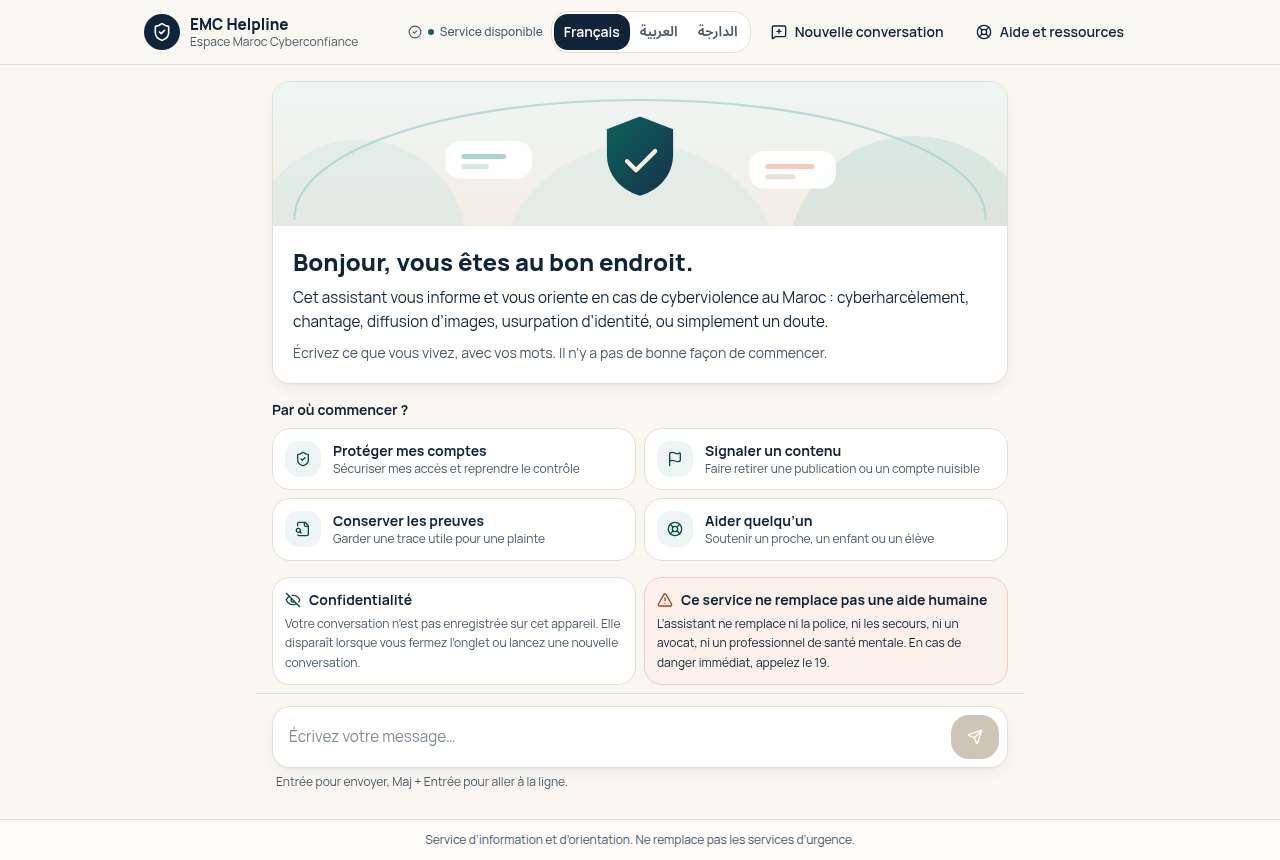
\includegraphics[width=0.94\textwidth]{figures/fig_accueil.png}
\caption{Écran d'accueil : présentation du service, avis de confidentialité,
rappel des limites et suggestions d'entrée en matière}
\label{fig:accueil}
\end{figure}

\begin{figure}[htbp]
\centering
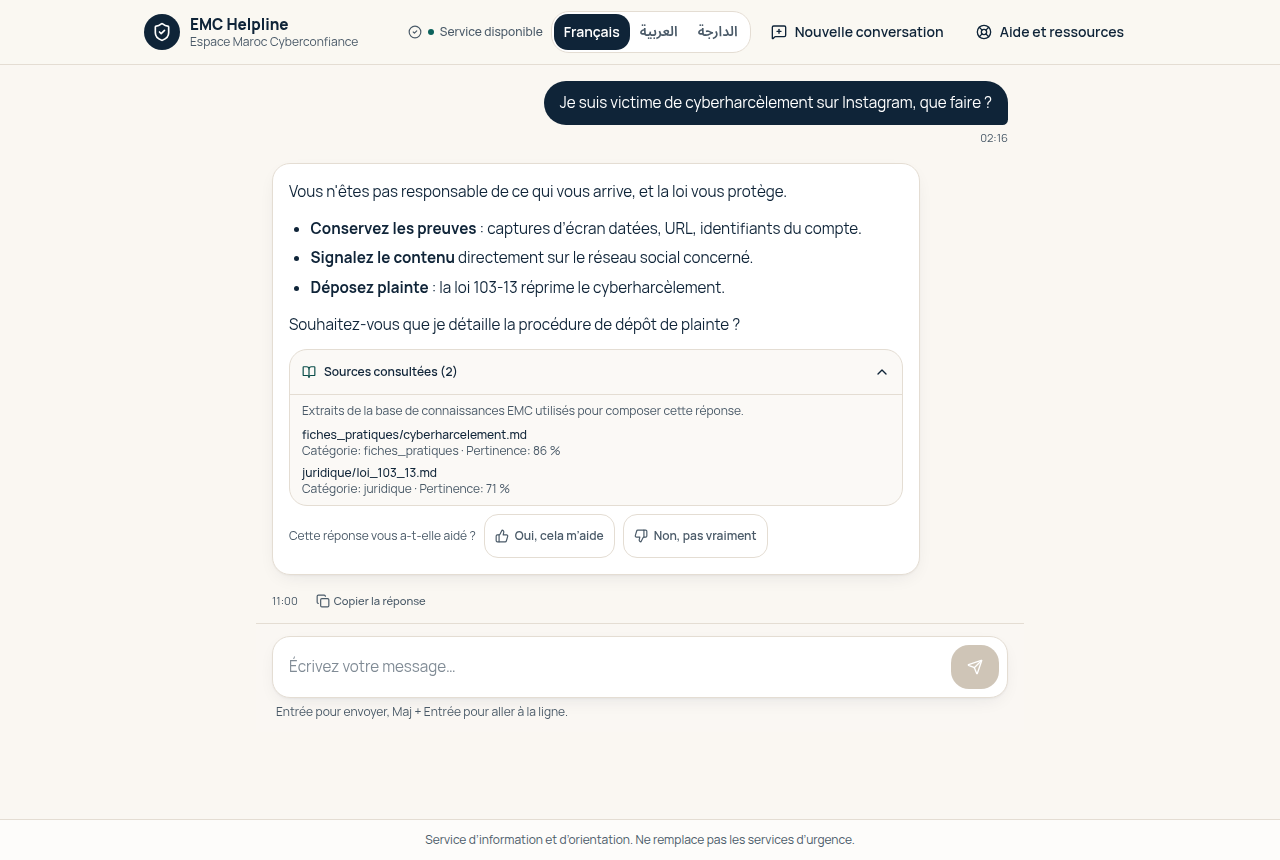
\includegraphics[width=0.94\textwidth]{figures/fig_conversation.png}
\caption{Conversation en français : réponse structurée et sources documentaires
consultées, dépliables à la demande}
\label{fig:conversation}
\end{figure}

\begin{figure}[htbp]
\centering
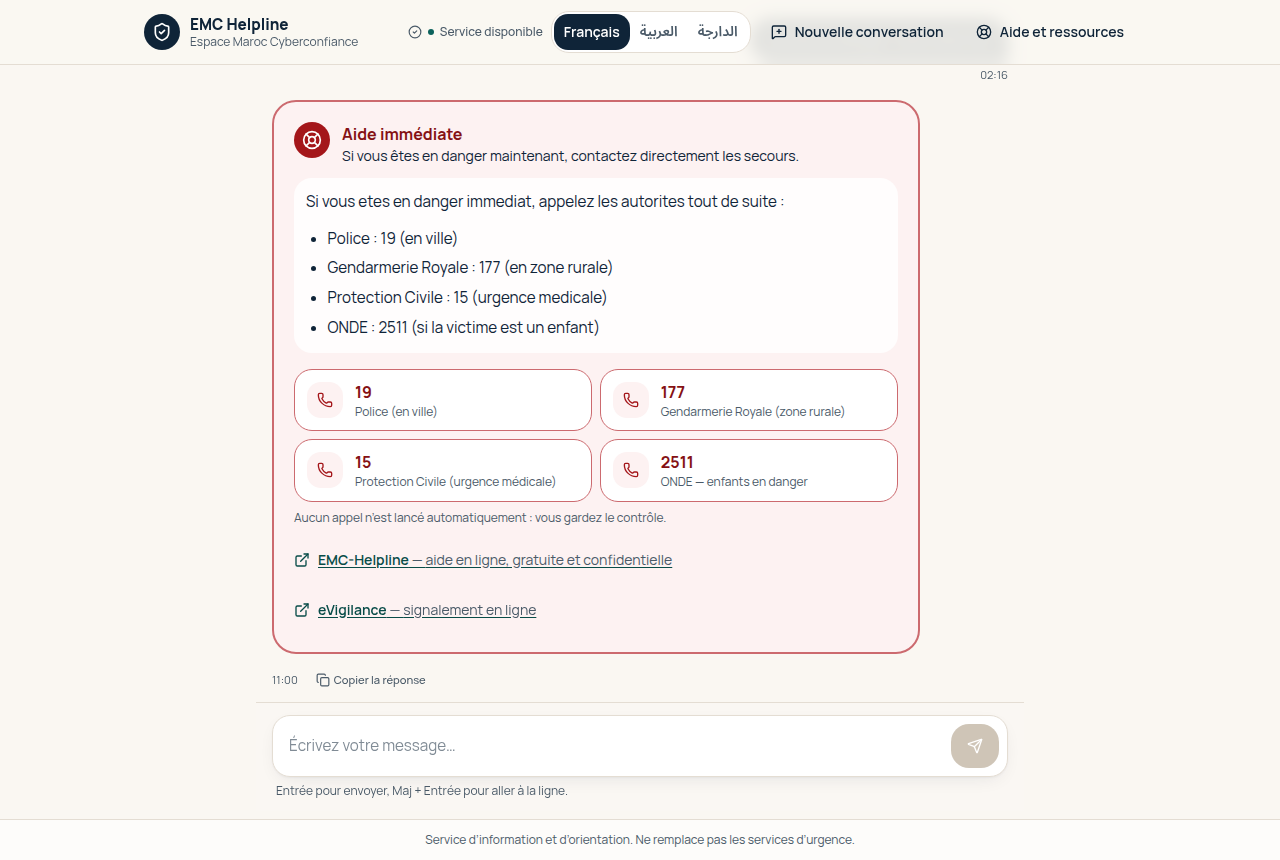
\includegraphics[width=0.94\textwidth]{figures/fig_urgence.png}
\caption{Protocole d'urgence : panneau annoncé aux lecteurs d'écran, numéros
officiels directement appelables, traitement visuel volontairement sobre}
\label{fig:urgence}
\end{figure}

\begin{figure}[htbp]
\centering
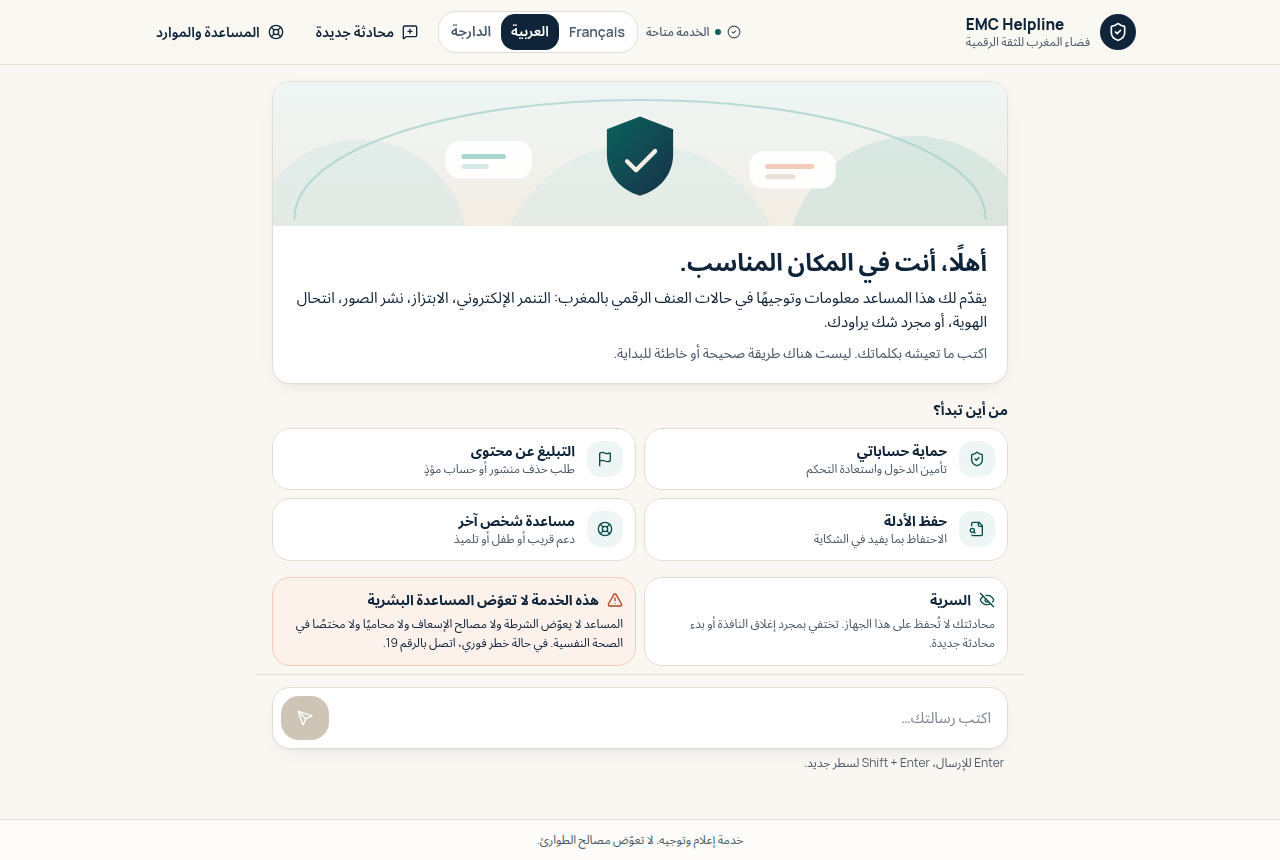
\includegraphics[width=0.94\textwidth]{figures/fig_arabe_rtl.png}
\caption{Interface en arabe : inversion complète de la mise en page (RTL),
tandis que les nombres et les identifiants latins conservent leur sens de lecture}
\label{fig:arabe}
\end{figure}

\begin{figure}[htbp]
\centering
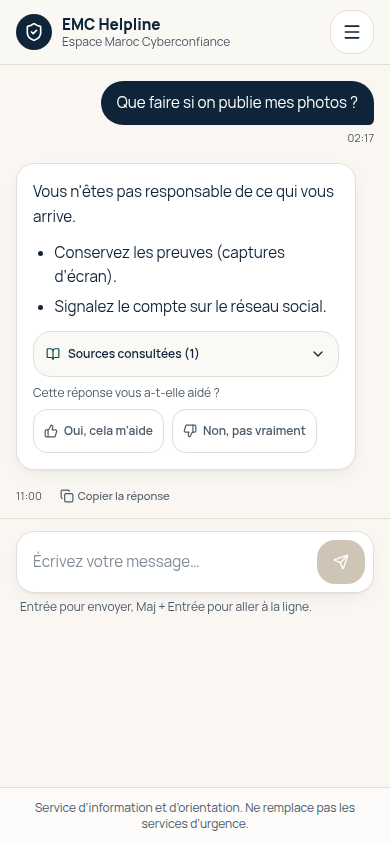
\includegraphics[width=0.42\textwidth]{figures/fig_mobile.png}
\caption{Affichage mobile : navigation repliée et zone de saisie toujours accessible}
\label{fig:mobile}
\end{figure}

\section{Accessibilité}

L'interface vise le niveau AA de la norme WCAG 2.2 : contrastes vérifiés
automatiquement sur les jetons de conception, navigation clavier complète,
zones d'annonce distinctes pour les réponses ordinaires
(\texttt{aria-live="polite"}) et pour les urgences (\texttt{role="alert"}),
respect de \texttt{prefers-reduced-motion}.

\section{Sécurité applicative}

\begin{itemize}[itemsep=2pt]
  \item Assainissement systématique du Markdown généré ; le HTML brut n'est
  jamais interprété.
  \item Liste blanche de schémas d'URL (\texttt{http}, \texttt{https},
  \texttt{mailto}, \texttt{tel}).
  \item Limitation de débit à 30 requêtes par minute et par adresse IP.
  \item Endpoints d'administration désactivés par défaut et protégés par clé.
  \item Aucune persistance du contenu des conversations côté navigateur.
\end{itemize}

% =====================================================================
\chapter{Tests, évaluation et déploiement}
\label{chap:validation}

\section{Stratégie de tests}

\begin{table}[htbp]
\centering
\small
\begin{tabular}{@{}lrp{6.4cm}@{}}
\toprule
\textbf{Suite} & \textbf{Tests} & \textbf{Portée} \\
\midrule
Backend (pytest)            & 170 & Ingestion, recherche, chaîne RAG, détection de langue, sessions, schémas, authentification \\
Frontend (Vitest)           & 100 & Client API, rendu, sécurité du Markdown, RTL, accessibilité (axe-core) \\
End-to-end (Playwright)     & 25  & Parcours complets sur navigateur, mobile et bureau \\
Scripts (pytest)            & 22  & Acquisition et normalisation des images \\
\midrule
\textbf{Total}              & \textbf{317} & \\
\bottomrule
\end{tabular}
\caption{Répartition des tests automatisés}
\label{tab:tests}
\end{table}

\section{Mesures}

\begin{table}[htbp]
\centering
\small
\begin{tabular}{@{}lr@{}}
\toprule
\textbf{Indicateur} & \textbf{Valeur mesurée} \\
\midrule
Vecteurs indexés (français / arabe) & 820 (535 / 285) \\
Documents ingérés                   & 122 \\
Latence de recherche vectorielle (médiane) & 19 ms \\
Latence du protocole d'urgence      & sans appel LLM \\
Code backend (hors tests)           & 3\,246 lignes \\
Code frontend (hors tests)          & 3\,417 lignes \\
Code de test                        & 3\,150 lignes \\
Poids du bundle frontend (gzip)     & 121 Ko \\
\bottomrule
\end{tabular}
\caption{Indicateurs mesurés sur le dépôt}
\label{tab:metrics}
\end{table}

\todo{Compléter par la latence de bout en bout mesurée en production
(\texttt{POST /api/chat}) sur un échantillon de requêtes réelles, et par les
résultats de la campagne d'évaluation qualitative des réponses.}

\section{Évaluation qualitative des réponses}

\todo{Reprendre et actualiser \texttt{docs/evaluation\_llm.md} : la matrice des
20 scénarios doit être ré-exécutée, d'une part parce que le modèle configuré a
changé, d'autre part parce que l'index arabe s'est enrichi de 72 fragments
supplémentaires.}

\section{Déploiement}

Le backend est déployé sur \emph{Hugging Face Spaces} (SDK Docker) et le
frontend sur \emph{Vercel}, deux offres gratuites. L'image du backend embarque le
modèle d'embeddings et construit la base vectorielle \emph{pendant la
construction}, ce qui garantit un démarrage déterministe. Le frontend relaie les
appels \texttt{/api} vers le backend, ce qui maintient l'ensemble sur une même
origine et permet de conserver une politique de sécurité de contenu stricte.

La procédure complète figure dans \texttt{docs/guide\_deploiement.md}.

\todo{Insérer l'URL publique de démonstration une fois le déploiement effectué.}

% =====================================================================
\chapter*{Conclusion et perspectives}
\addcontentsline{toc}{chapter}{Conclusion et perspectives}
\markboth{Conclusion et perspectives}{}

\todo{Rédiger la conclusion : rappel des objectifs, bilan de ce qui a été
réalisé, apports personnels et compétences acquises, difficultés rencontrées.}

\section*{Perspectives}

\begin{enumerate}[itemsep=2pt]
  \item \textbf{Couverture de l'arabizi dans la détection d'urgence.} Les
  marqueurs de danger vital ne sont actuellement définis qu'en caractères
  arabes ; leur transcription latine doit être ajoutée pour couvrir les
  utilisateurs écrivant la darija en caractères latins.
  \item \textbf{Persistance des sessions.} Le passage à un magasin Redis
  permettrait de survivre aux redémarrages et de répartir la charge sur
  plusieurs instances.
  \item \textbf{Embeddings distants.} Le recours à une API d'embeddings
  allégerait considérablement l'image de déploiement, au prix d'un recalibrage
  du seuil de similarité.
  \item \textbf{Enrichissement de la base arabe.} Le corpus arabe reste moins
  fourni que le corpus français (285 vecteurs contre 535).
  \item \textbf{Évaluation avec des utilisateurs réels}, encadrée sur le plan
  éthique, afin de mesurer l'utilité perçue du dispositif.
\end{enumerate}

% =====================================================================
\chapter*{Bibliographie et webographie}
\addcontentsline{toc}{chapter}{Bibliographie et webographie}
\markboth{Bibliographie et webographie}{}

\begin{enumerate}[itemsep=2pt,label={[\arabic*]}]
  \item Espace Maroc Cyberconfiance (EMC) — \url{https://www.cyberconfiance.ma}
  \item Plateforme nationale de signalement eVigilance — \url{https://evigilance.ma}
  \item Royaume du Maroc, \emph{Loi n\textsuperscript{o} 103-13 relative à la lutte contre les violences faites aux femmes}.
  \item Royaume du Maroc, \emph{Loi n\textsuperscript{o} 07-03 complétant le code pénal en ce qui concerne les infractions relatives aux systèmes de traitement automatisé des données}.
  \item Royaume du Maroc, \emph{Loi n\textsuperscript{o} 09-08 relative à la protection des personnes physiques à l'égard du traitement des données à caractère personnel}.
  \item P. Lewis \emph{et al.}, \emph{Retrieval-Augmented Generation for Knowledge-Intensive NLP Tasks}, NeurIPS, 2020.
  \item N. Reimers, I. Gurevych, \emph{Sentence-BERT: Sentence Embeddings using Siamese BERT-Networks}, EMNLP, 2019.
  \item W3C, \emph{Web Content Accessibility Guidelines (WCAG) 2.2}, 2023.
\end{enumerate}

\todo{Compléter avec les rapports UNICEF, UNESCO, OMS et Conseil de l'Europe
effectivement exploités dans la base de connaissances.}

% =====================================================================
\appendix
\chapter{Annexes}

\section{Numéros d'urgence intégrés}

\begin{table}[htbp]
\centering
\small
\begin{tabular}{@{}llp{5.6cm}@{}}
\toprule
\textbf{Service} & \textbf{Numéro} & \textbf{Portée} \\
\midrule
Police secours          & 19   & Zones urbaines, 24h/24 \\
Gendarmerie Royale      & 177  & Zones rurales, 24h/24 \\
Protection Civile       & 15   & Urgence médicale \\
ONDE                    & 2511 & Enfants en danger, gratuit \\
EMC-Helpline            & ---  & \url{https://www.cyberconfiance.ma} \\
eVigilance              & ---  & \url{https://evigilance.ma/fr/signaler} \\
\bottomrule
\end{tabular}
\caption{Dispositifs d'urgence et de signalement intégrés au système}
\label{tab:urgence}
\end{table}

\section{Structure du dépôt}

\begin{lstlisting}[language=bash,caption={Organisation des sources},label={lst:arbo}]
backend/          API FastAPI et pipeline RAG
  api/            routes, schemas, middlewares, securite
  llm/            fournisseur Gemini
  prompts/        prompts systeme FR et AR
  rag/            ingestion, embeddings, retriever, chain
  services/       langue, sessions, orchestration
frontend/         interface React + TypeScript
data/             base de connaissances et base vectorielle
docs/             livrables, analyses, guide de deploiement
plan/             planification des quatre sprints
\end{lstlisting}

\section{Exemple de réponse en situation d'urgence}

\begin{lstlisting}[caption={Réponse renvoyée sans appel au modèle de langage},label={lst:urgence}]
Si vous etes en danger immediat, appelez les autorites tout de suite :
- Police : 19 (en ville)
- Gendarmerie Royale : 177 (en zone rurale)
- Protection Civile : 15 (urgence medicale)
- ONDE : 2511 (si la victime est un enfant)
- EMC-Helpline : cyberconfiance.ma (en ligne, gratuit)

Vous n'etes pas seul(e). L'aide est disponible 24h/24.
\end{lstlisting}

\end{document}
